with steps per year: 7*3600*360
Running velocity verlet
Perihelion position after 100 years: 0.307498, -0.000933806
Perihelion angle after 100 years: -626.38 arc seconds
CPU time: 3248.07


Result:		
	- Find out which initial velocity that gives a circular motion (plot)
\begin{figure}[H]
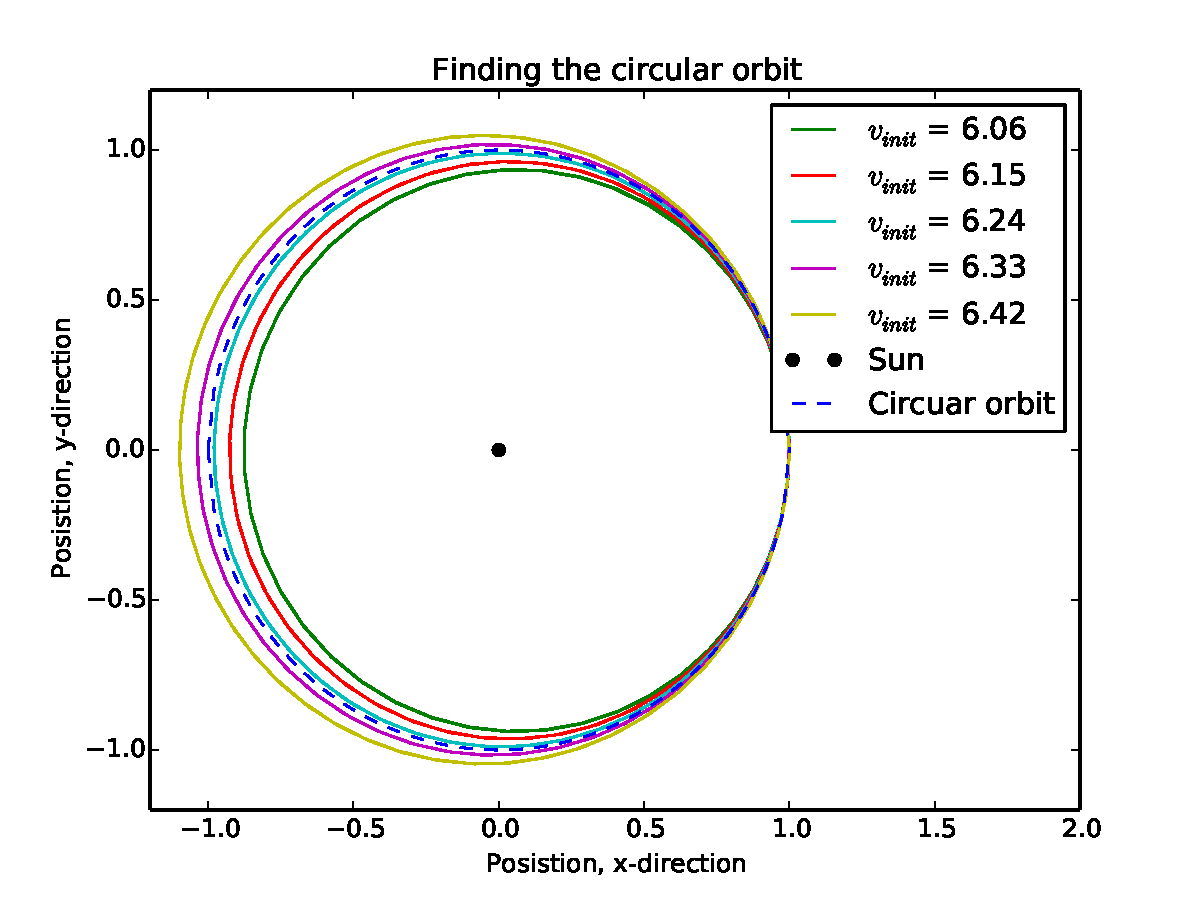
\includegraphics[width=1.1\linewidth]{../results/plots/circular_orbit.pdf}\caption{This is a plt of the orbit with different initial velocities. The circular orbit has a velocity between 6.24 and 6.33. $2 \pi = 6.28$ and that is the initial velocity that gives a circular orbit. }\label{fig:circular_orbit}
\end{figure}

	- Test stability (energy-stability) as function of dt (both Verlet and Euler)
	- Plot the earth orbiting the sun
	- Check (for the circular orbit) that the energy is conserved (plot - both kin and pot separated and together?)
	- Check that angular moment is conserved

	- Find escape velocity (plot)
	 	- Compare exact and numerical results
	- Find exact escape velocity (theory?)
	- Changing beta (plot)
		- Comment result + What happens when beta -> 3 ? (last part in discussion?
	- How much does Jupiter alter Earth's orbit?
	- Position of Jupiter and Earth (plot)	
	- Plot Earth's motion for increased mass of Jupiter (3 masses)
	- Find center off mass - use as origin
	- Give sun initial velocity so momentum is zero (origin is fixed)
	- Compare with 3e)
	- Extend to all planets (plot)
	- Find perihelion for both relativistic and non-relativisitc (table)
	- Relativistic - should be a few magnitudes smaller.	
	-  Can the observed perihelion
precession of Mercury be explained by the general theory of relativity?
